\chapter{Task 44}

\resp{Asal Kermaniha}

\subsection{Introduction}
In this task, we construct networks based on word co-occurrences for eleven languages. First, 11 languages were selected from the language column of the downloaded metadata file \cite{keruiduo_supp}. Here is a list of these languages:” Finnish, Hungarian, Turkish, Serbian, English, Italian, German, French, Spanish, Catalan, Basque”. All of the languages are selected considering them to have white space separating the words in the sentence in order to avoid complexity in preprocessing level. Second, the data were downloaded from the recommended source\cite{leipzig_corpora}.
\subsection{Data and preprocessing}
 After the files were downloaded, the sentence file was extracted from each dataset. The sentence file included 10k/30k lines, each containing a single sentence.

\noindent
The meta data also contained the following columns and information:

\noindent
\textbf{Duration:} Time required to read the text, measured in seconds.

\noindent
\textbf{NS:} Number of canonical syllables in the text. 

\noindent
\textbf{ShE:} Shannon entropy of the language, computed from the distribution of syllables. (measuring the average uncertainty associated with observing a syllable in that language.)

\noindent
\textbf{ID:} Information density, measuring how much information is conveyed per syllable. 

\noindent
All lines of each file are read; same number of sentences (5k due to computational limitation. later I increased the amount to 7000 for robustness test) is selected from each file. The number in the beginning of each sentence is omitted, all the letters are turned into lowercase, punctuation signs are replaced with space, and then multiple spaces are unified. finally, each word of every single line is separated as a single string. The final output of the function is a list of vectors. Each vector corresponds to a sentence, and inside it we have the separated words of the sentence.

\noindent
The frequency of each word is then computed across all selected sentences in each corpus. The words are then sorted according to their frequencies and a unique ID is assigned to each word, with the most frequent word receiving the lowest ID. Only words with a frequency greater than or equal to 2 are retained. The output of this step is a data frame containing the selected words and their corresponding IDs.

\noindent
After all, the output of the last two paragraphs is integrated. which interprets the output of the former step in a list of vectors which still contains the same sentences but within the vectors each word is replaced with its ID which was in the second step’s output.

\subsection{Network Construction}
For each line in the file, a loop is defined that searches the sentence word by word, starting from the first word, and builds an edge between the current word and any word located within the radius \texttt{window\_size} = 2. Since the network is undirected, the lowest ID is always considered the source node. The output of this function is a data frame containing two columns, \texttt{from} and \texttt{to}, which store node IDs as values in each row. Each row corresponds to an edge in the network.

\noindent
The weight of each edge is then computed by counting its occurrences in the data frame. All edges with a weight greater than zero are retained. The resulting weights are added as a new column to the output of the previous step.

\noindent
Finally, a graph object is defined, in which word IDs are used as nodes and weighted edges represent word co-occurrences.
For each language, a node file and an edge file are generated. Both files are saved in CSV format and contain the following columns:

\texttt{node\_df}: [``word'', ``frequency'', ``wordID'', ``language'']

\texttt{weight\_df}: [``from'', ``to'', ``weight'', ``language'']

\subsection{Network Analysis}

degree distribution and strength distribution are both visualized for each language. results for the English language have been presented as a sample in figure 2.2

\noindent
A high degree does not necessarily mean that a word is used frequently. Instead, it indicates the number of distinct words with which it co-occurs. Therefore, a node of high degree is connected to many different words. while, the strength distribution signifies the actual frequency of these co-occurrences and provides a measure of how often a word is used within the network. As demonstrated in Figure 2.2, both degree and strength distributions exhibit a power-law-like behavior for all of the languages studied. This means that in both distributions there are many low degree and strength nodes and a few high degree and strength ones.

\noindent
Using the \texttt{igraph} library, the main graph properties were computed for each language network. The results were stored in a data frame named \texttt{network\_summary.csv}, whose columns are as follows:

\begin{flushleft}
\texttt{["nodes", "edges", "density", "mean\_degree", "max\_degree", "components", "largest\_component", "clustering\_coefficient", "assortativity", "modularity"]}
\end{flushleft}

\noindent
According to this table, each node has one connected component; this means that all the studied words are connected as a single component. Visualization is also provided in Figure 2.1.


\begin{figure}[H]
\centering

\begin{tabular}{ccc}

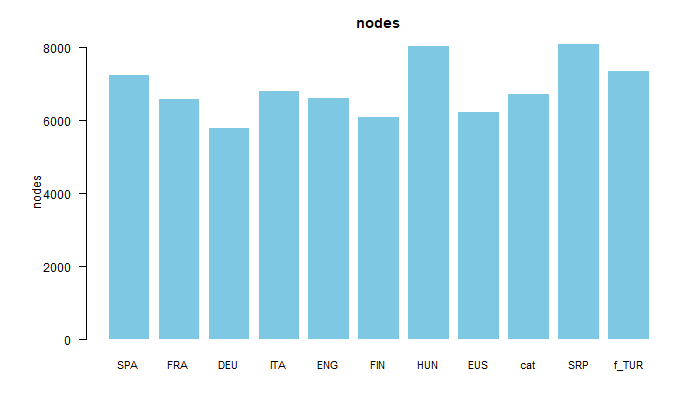
\includegraphics[width=0.28\textwidth]{images/computational_project_results/table_graphs/nodes.png} &
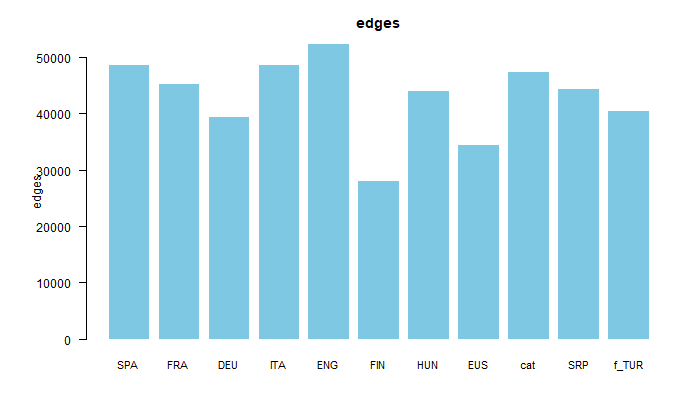
\includegraphics[width=0.28\textwidth]{images/computational_project_results/table_graphs/edges.png} &
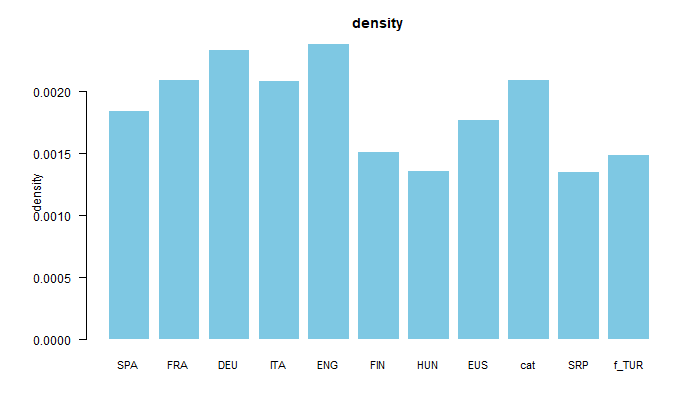
\includegraphics[width=0.28\textwidth]{images/computational_project_results/table_graphs/density.png} \\

Nodes & Edges & Density \\[2mm]

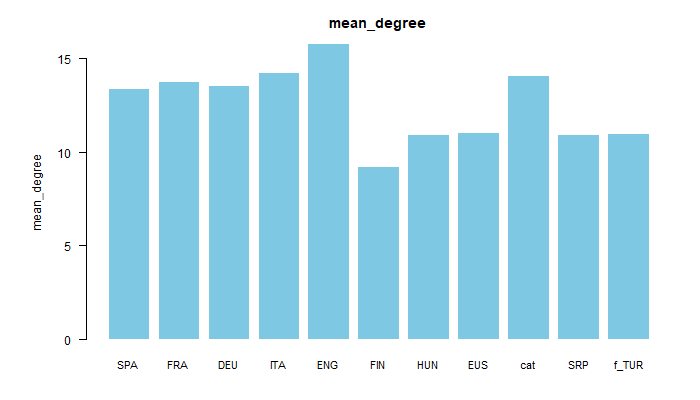
\includegraphics[width=0.28\textwidth]{images/computational_project_results/table_graphs/mean_degree.png} &
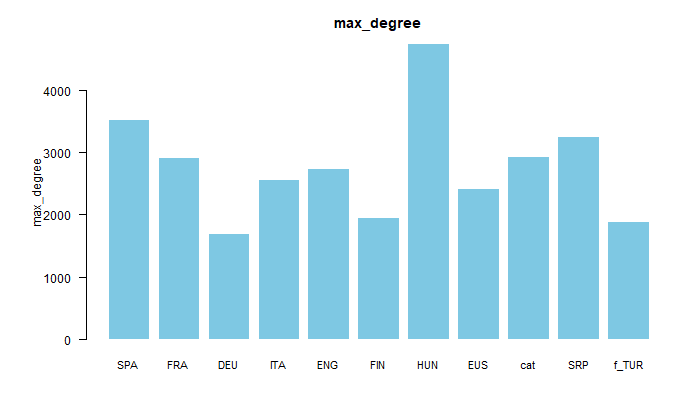
\includegraphics[width=0.28\textwidth]{images/computational_project_results/table_graphs/max_degree.png} &
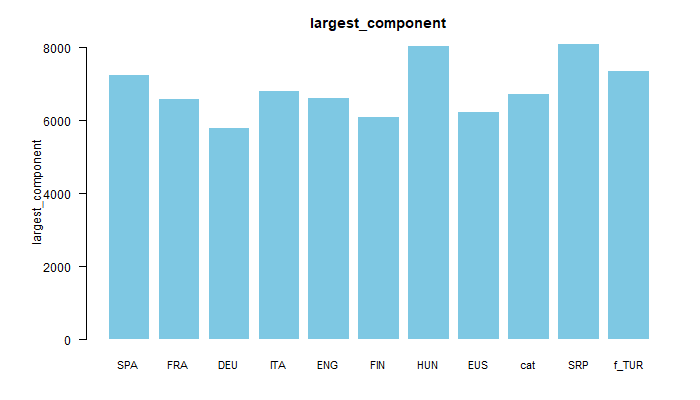
\includegraphics[width=0.28\textwidth]{images/computational_project_results/table_graphs/largest_component.png} \\

Mean Degree & Max Degree & Largest Component \\[2mm]

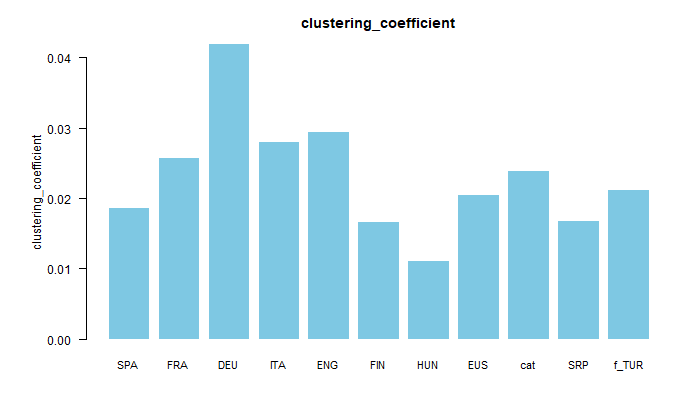
\includegraphics[width=0.28\textwidth]{images/computational_project_results/table_graphs/clustering_coefficient.png} &
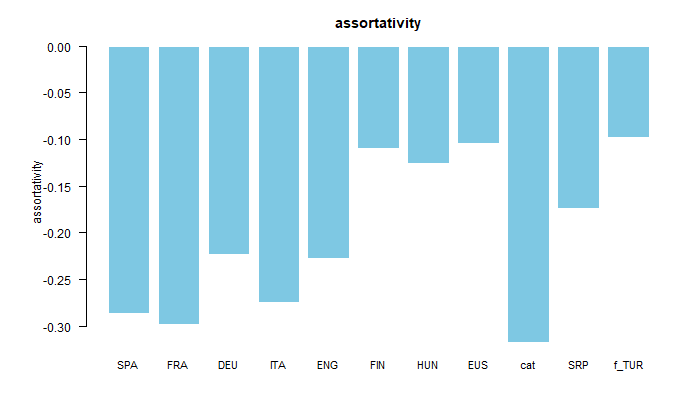
\includegraphics[width=0.28\textwidth]{images/computational_project_results/table_graphs/assortativity.png} &
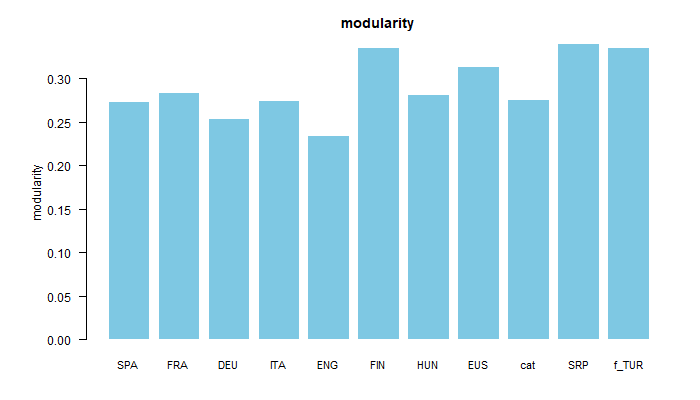
\includegraphics[width=0.28\textwidth]{images/computational_project_results/table_graphs/modularity.png} \\

Clustering & Assortativity & Modularity

\end{tabular}

\caption{Comparison of network properties across languages.
\newline
*Modularity was computed after detecting communities using the Louvain algorithm.
}
\label{fig:network_properties}

\end{figure}



\begin{figure}[htbp]
\centering

\begin{minipage}[t]{0.50\textwidth}
\centering
\textbf{(a)}\\[2mm]
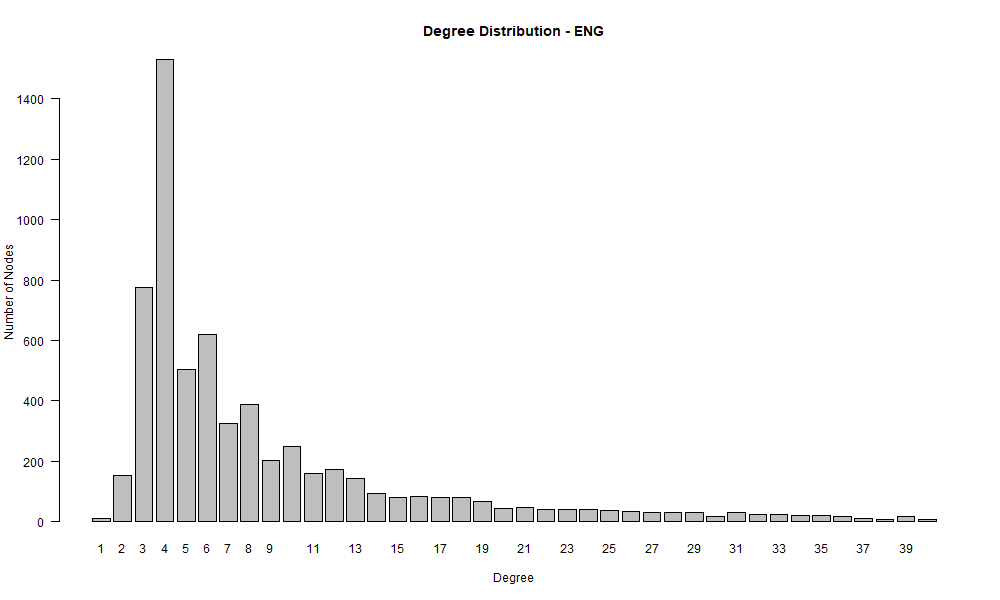
\includegraphics[width=\linewidth]{images/computational_project_results/distributions/node_dist/ENG_degree_distribution.png}
\end{minipage}
\hfill
\begin{minipage}[t]{0.41\textwidth}
\centering
\textbf{(b)}\\[2mm]
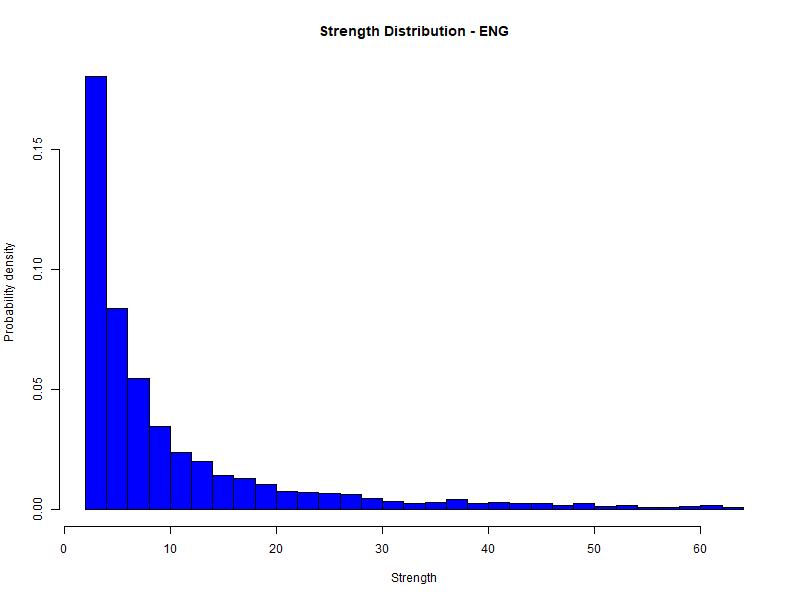
\includegraphics[width=\linewidth]{images/computational_project_results/distributions/strength_dist/ENG_strength_distribution.png}
\end{minipage}

\caption{power-law-like behavior of degree (a) and strength(b) distributions for the English word co-occurrence network.(as a sample). other language's plots are available in images}
\label{fig:degree_strength_dist}

\end{figure}

\noindent
As we are dealing with sparse networks, we know that the more crowded the networks, the smaller the density. Higher network density increases the probability that neighbors of a node are connected to each other, leading to the formation of more triangles, and consequently a higher clustering coefficient.


\noindent
keeping an eye to degree distribution, we can see that languages which have heavier tails have a higher mean degree, which is not surprising because they have more hubs. consequently, languages with higher mean degrees have lower modularity because hubs tend to connect different modules to each other. All languages are disassortative, which means that hubs tend to connect lower degree nodes more than other hubs, but according to scale-free degree distribution, there is a possibility that this diassortativity could be a consequence of topological limitations. we have to do further analysis on null model to validate these results and see if they are caused by degree distribution.

\noindent
since networks have one component each, we can see the exact same pattern of nodes plot in the largest component's size plot.

\noindent

\subsection{correlation analysis}

The metadata data frame was filtered to retain only the selected languages. The relevant rows and numeric variables were extracted and the average value of repeated observations was computed for each language. 


\noindent
Subsequently, the metadata table and the \texttt{network\_summary} table were merged into a single file named \texttt{merged.csv}.

\noindent
To investigate the relationship between information-theoretic variables and network descriptors, Spearman rank correlation coefficients were computed. The Spearman correlation was preferred because it can capture monotonic relationships without assuming linear dependence between variables.

\noindent
The results show that some of the information theory variables have similar behavior as network descriptors, which is described as following:


\begin{figure}[H]
\centering

\begin{minipage}[t]{0.47\textwidth}
\centering
\textbf{(a)}\\[2mm]
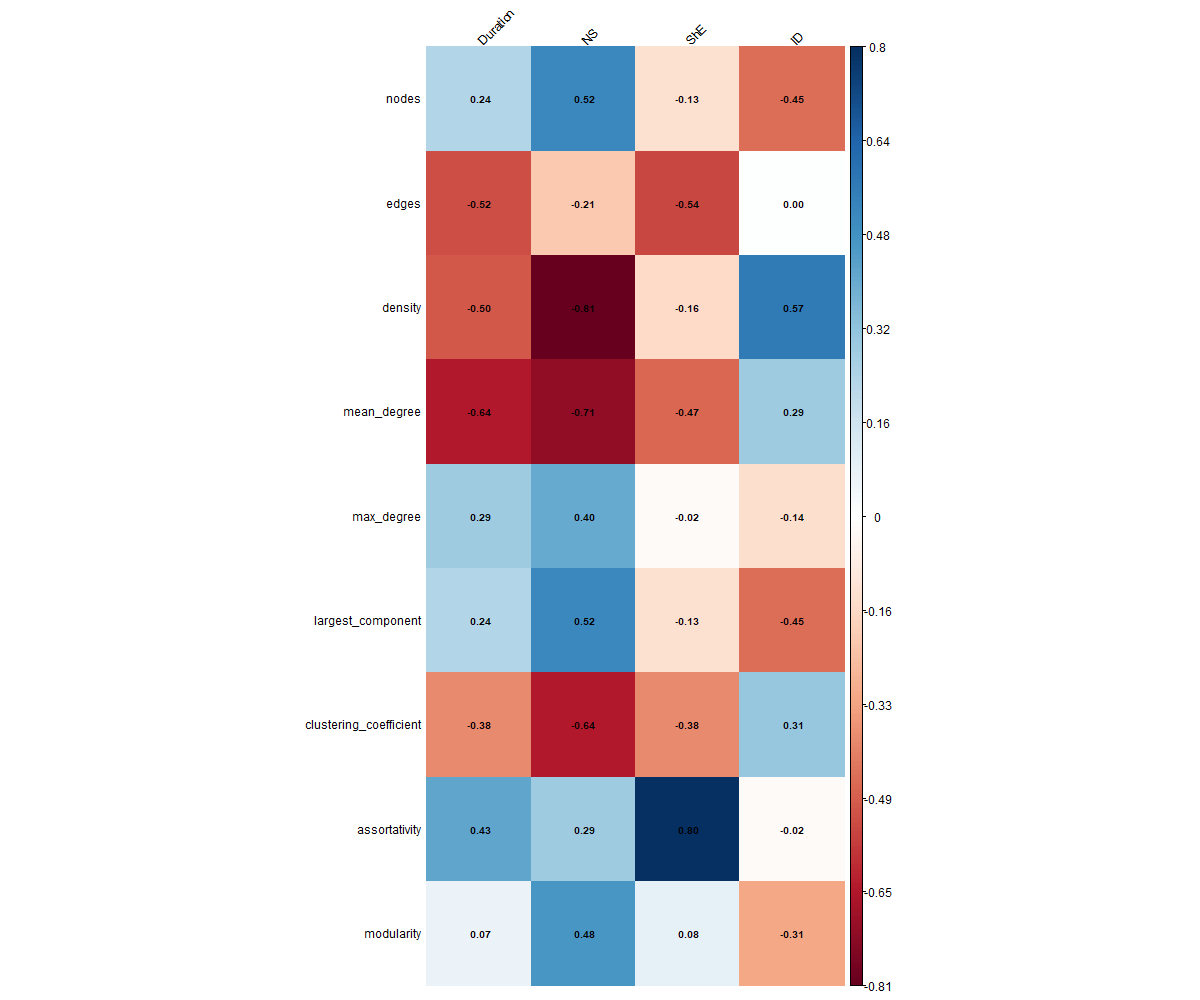
\includegraphics[width=\linewidth]{images/computational_project_results/correlation/spearman_correlation_matrix.png}
\end{minipage}
\hfill
\begin{minipage}[t]{0.47\textwidth}
\centering
\textbf{(b)}\\[2mm]
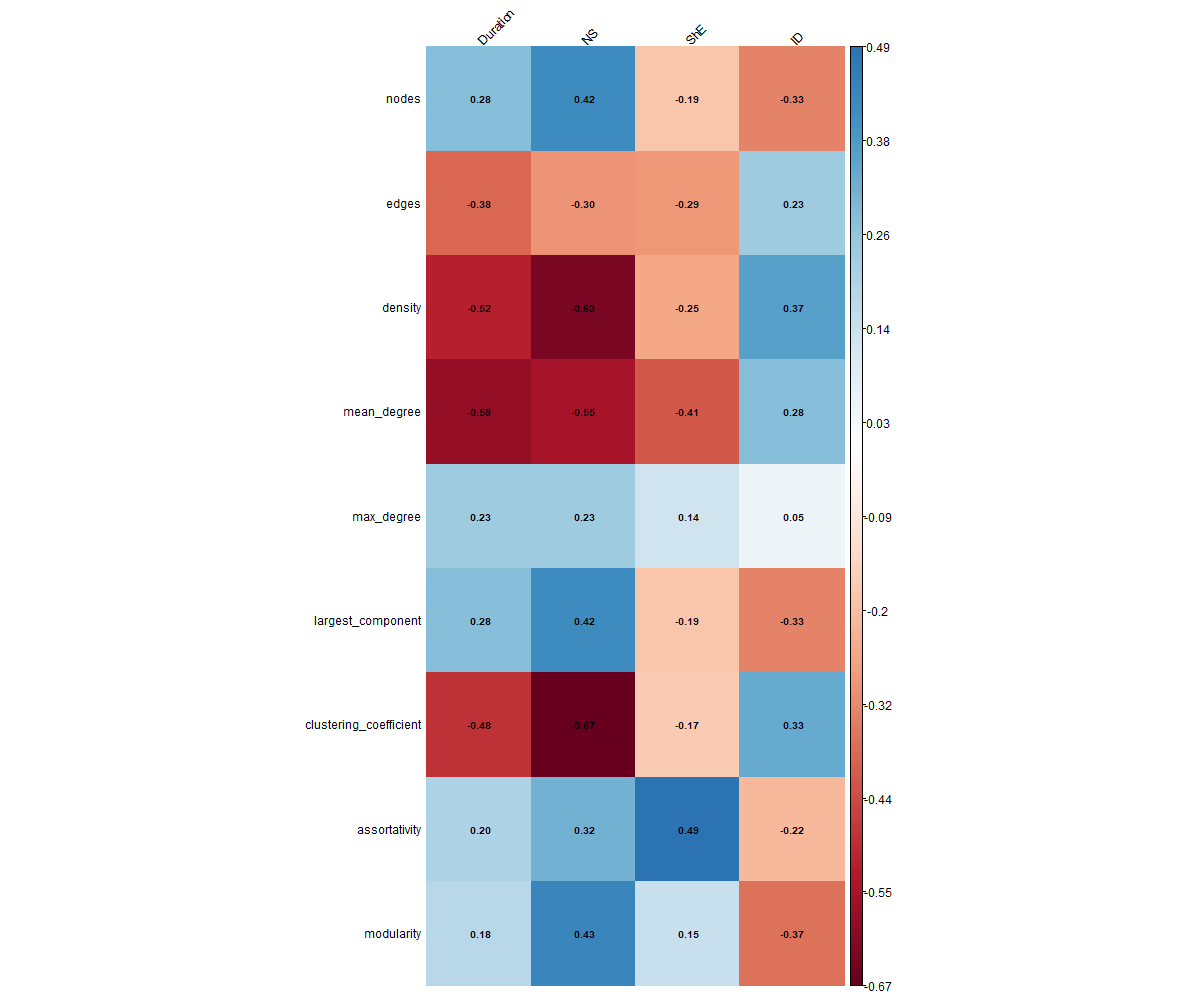
\includegraphics[width=\linewidth]{images/computational_project_results/correlation/spearman_correlation_matrix_robustness.png}
\end{minipage}

\caption{correlation matrix window size=2(a) robustness check window size=3(b)
\newline increasing the co-occurrence window from 2 to 3 caused a slight change in the magnitude of several correlations since Metrics such as density, mean degree, clustering coefficient and modularity are sensitive to network construction choices
}
\label{fig:degree_strength_dist}

\end{figure}

\noindent
Duration and Number of Syllables (NS) are both negatively associated with density and mean degree, while showing positive correlations with modularity and assortative. That means that once the words have more syllables, they take longer time to be told, and they usually do not co-occur with any other word out of their own module. This indicates that languages requiring more syllables and longer speaking times tend to have sparser word co-occurrence networks.

\noindent
Information Density (ID) displays an almost opposite pattern. This difference is explainable once we know that the larger number of syllables means having less amount of information (ID) per each. Positive correlations with density, mean degree, and clustering coefficient suggest that languages with higher information density tend to exhibit more locally interconnected network structures. At the same time, the negative correlation with modularity indicates a weaker separation between network communities.

\noindent
Shannon entropy correlations are less robust compared to NS and ID. However, they become stronger when the window size is increased from 2 to 3.This means that, in order to perform a more precise analysis of this variable's correlations, we may need to consider broader word interactions rather than only local interactions. 

\subsection{methodological limitations}
Several methodological limitations should be considered when interpreting these results. 
The same preprocessing procedure was applied to all language; However,  Punctuation, numbers, and formatting symbols were removed, and all words were converted to lowercase. Although these choices simplify the analysis and improve comparability across languages, they may also remove linguistic information.

\noindent
Due to computational limitations, only a subset of 5000/7000 sentences was used for each language. Consequently, reconstructed networks may not fully capture the complete lexical and structural diversity of the original corpora.

\noindent
stop words were not removed, while they can have some effects on network descriptors once they are used frequently.

\noindent
The same type of corpus was used for all languages(other than EUS cause news corpus was not available for that one). However, results may be sensitive to corpus types.

\noindent
Languages without whitespace segmentation were not included in this study and they have to go through a different preprocessing procedure.





